% =====================================================================
%  Лабораторная работа №5. Методы решения дифференциальных уравнений.
%  Вариант 4: 3*y*y' = 2*x, y(-2) = -3; отрезок [-2; -1].
%
%  Сборка (любой из вариантов):
%      pdflatex  BastrakovReport.tex
%      xelatex   BastrakovReport.tex
%      lualatex  BastrakovReport.tex
%  (запускать два раза — для оглавления и перекрёстных ссылок)
% =====================================================================
\documentclass[14pt,a4paper]{extarticle}

% - Поддержка кириллицы: pdfLaTeX (T2A) либо XeLaTeX/LuaLaTeX (fontspec) -
\usepackage{iftex}
\ifPDFTeX
    \usepackage[T2A]{fontenc}
    \usepackage[utf8]{inputenc}
    \usepackage[russian]{babel}
    \usepackage{tempora}
    \usepackage{listingsutf8}
\else
    \usepackage{fontspec}
    \usepackage{polyglossia}
    \setdefaultlanguage{russian}
    \setotherlanguage{english}
    \IfFontExistsTF{Liberation Serif}%
        {\setmainfont{Liberation Serif}}%
        {\IfFontExistsTF{PT Serif}%
            {\setmainfont{PT Serif}}%
            {\setmainfont{TeX Gyre Termes}}}
    \IfFontExistsTF{DejaVu Sans Mono}%
        {\setmonofont{DejaVu Sans Mono}}%
        {\IfFontExistsTF{Liberation Mono}%
            {\setmonofont{Liberation Mono}}%
            {\setmonofont{TeX Gyre Cursor}}}
\fi

% - Математика, графика, оформление -----------
\usepackage{amsmath,amssymb}
\usepackage{graphicx}
\usepackage{geometry}
\usepackage{booktabs}
\usepackage{array}
\usepackage{float}
\usepackage{caption}
\usepackage{indentfirst}
\usepackage{xcolor}
\usepackage[hidelinks]{hyperref}

\geometry{a4paper,left=3cm,right=1.5cm,top=2cm,bottom=2cm}
\graphicspath{{graphics/img/}}

\captionsetup{labelsep=endash,justification=centering}
\setlength{\parindent}{1.25cm}
% Запас на растяжение строк: в XeLaTeX могут отсутствовать русские
% шаблоны переносов, поэтому длинные слова иначе вылезают за поля.
\setlength{\emergencystretch}{3em}
\tolerance=2000
\renewcommand{\arraystretch}{1.15}
\renewcommand{\labelenumi}{\arabic{enumi})}

\begin{document}

% =====================================================================
%  Титульный лист
% =====================================================================
\begin{titlepage}
    \centering
    \large
    Министерство образования и науки РФ\\[0.3cm]
    Пермский национальный исследовательский политехнический университет\\[0.3cm]
    Электротехнический факультет\\[0.3cm]
    Кафедра "Информационные технологии и автоматизированные системы"

    \vspace{3.5cm}
    {\Large Информатика в приложении к отрасли}\\[0.4cm]
    {\Large\bfseries Лабораторная работа № 5}\\[0.6cm]

    Тема: "Методы решения дифференциальных уравнений"\\[0.2cm]
    Вариант 4

    \vspace{4.5cm}
    \begin{flushleft}
        \large
        Выполнил: студент группы РИС-25-2б \hfill Бастраков Данил\\[0.5cm]
        Проверил: профессор кафедры ИТАС \hfill Шварц К.~Г.\\[0.5cm]
        Дата: \underline{\hspace{3cm}} \hfill Подпись: \underline{\hspace{4cm}}
    \end{flushleft}

    \vfill
    Пермь\\ 2026
\end{titlepage}

\tableofcontents
\newpage

% =====================================================================
\section{Постановка задачи}
% =====================================================================

\textbf{Цель работы} --- численно решить задачу Коши для обыкновенного
дифференциального уравнения первого порядка, реализовать выбранный метод
в программе и оценить погрешность решения с помощью принципа Рунге.

Вариант~4 задаёт уравнение и начальное условие
\begin{equation}
    3y y' = 2x, \qquad y(-2) = -3 .
    \label{eq:cauchy}
\end{equation}
Отрезок интегрирования согласно заданию равен $[x_0; x_0+1] = [-2;\, -1]$,
шаги сетки $h_1=0{,}1$ и $h_2=0{,}05$.

Номер варианта $N=4$, поэтому $N \bmod 5 = 4$: согласно заданию
используется \textbf{метод Рунге-Кутта четвёртого порядка}.

Для проверки численного решения найдём точное решение уравнения
\eqref{eq:cauchy}. Разделим переменные:
\[
    3y\,dy = 2x\,dx \quad\Longrightarrow\quad
    \frac{3}{2}y^2 = x^2 + C .
\]
Из начального условия $y(-2)=-3$ получаем
$\frac{3}{2}\cdot 9 = 4 + C$, то есть $C = \frac{19}{2}$. Следовательно,
$y^2 = \dfrac{2x^2+19}{3}$; отрицательная ветвь выбрана по начальному
условию:
\begin{equation}
    y(x) = -\sqrt{\frac{2x^2+19}{3}} .
    \label{eq:exact}
\end{equation}
В конце отрезка точное решение равно
\begin{equation}
    y(-1) = -\sqrt{7} = -2{,}6457513110645907 .
    \label{eq:exact-end}
\end{equation}
Правая часть уравнения, используемая в численном методе,
\begin{equation}
    y' = f(x,y) = \frac{2x}{3y} .
    \label{eq:rhs}
\end{equation}
На отрезке $[-2;\,-1]$ решение отрицательно и отделено от нуля, поэтому
правая часть \eqref{eq:rhs} определена и непрерывно дифференцируема:
метод Рунге-Кутта применим.

% =====================================================================
\section{Краткое описание метода}
% =====================================================================

\subsection{Метод Рунге-Кутта четвёртого порядка}

На равномерной сетке $x_i = x_0 + ih$ приближённые значения искомой
функции находятся по формуле
\begin{equation}
    y_{i+1} = y_i + \Delta y_i, \qquad
    \Delta y_i = \frac{1}{6}\left(K_0 + 2K_1 + 2K_2 + K_3\right),
    \label{eq:rk4}
\end{equation}
где
\begin{equation}
    \begin{aligned}
        K_0 &= h f(x_i, y_i),\\
        K_1 &= h f\!\left(x_i + \frac{h}{2},\ y_i + \frac{K_0}{2}\right),\\
        K_2 &= h f\!\left(x_i + \frac{h}{2},\ y_i + \frac{K_1}{2}\right),\\
        K_3 &= h f\!\left(x_i + h,\ y_i + K_2\right).
    \end{aligned}
    \label{eq:rk4-k}
\end{equation}
Погрешность на одном шаге имеет порядок $O(h^5)$, суммарная погрешность
на отрезке --- $O(h^4)$. Метод не требует вычисления производных правой
части и является явным: каждое следующее значение выражается через
уже известное $y_i$ и четыре вычисленные величины $K_0,\ldots,K_3$.

\subsection{Геометрическая интерпретация}

Решение задачи Коши --- интегральная кривая $y=\varphi(x,C_0)$, проходящая
через точку $(x_0,y_0)$; в каждой точке $(x,y)$ её касательная имеет
наклон $f(x,y)$. Метод Эйлера заменяет кривую на шаге одной касательной,
проведённой в левой точке, поэтому быстро накапливает ошибку.
Метод Рунге-Кутта вычисвает наклоны в четырёх точках шага: в начале,
дважды в середине и в конце. Средневзвешенное значение этих наклонов
(веса $1/6,\ 1/3,\ 1/3,\ 1/6$) учитывает изменение производной внутри
шага, благодаря чему ломаная ближе к интегральной кривой.

\subsection{Оценка погрешности. Правило Рунге}

Пусть получены два приближения в одной точке $x$: $y_h$ с шагом $h$ и
$y_{h/2}$ с шагом $h/2$. Для метода порядка $k$ полная погрешность
оценивается формулой
\begin{equation}
    y(x) \approx y_{h/2} + \frac{y_{h/2} - y_h}{2^k - 1} .
    \label{eq:runge}
\end{equation}
Для метода Рунге-Кутта $k=4$, поэтому знаменатель равен $2^4-1=15$:
\begin{equation}
    y(x) \approx y_{h/2} + \frac{y_{h/2} - y_h}{15} .
    \label{eq:runge4}
\end{equation}
Сетка с шагом $0{,}05$ содержит все узлы сетки с шагом $0{,}1$, поэтому
сравнение проводится непосредственно в общих узлах $x=-2{,}0;\,-1{,}9;
\,\ldots;\,-1{,}0$.

% =====================================================================
\section{Исходные данные}
% =====================================================================

Программа читает параметры из файла \texttt{input.txt}; комментарии
начинаются с символа~\texttt{\#}. Файл содержит пять чисел:
$x_0,\ x_1,\ y_0,\ h_1,\ h_2$. Для варианта~4:
\begin{equation}
    x_0 = -2,\qquad x_1 = -1,\qquad y_0 = -3,\qquad
    h_1 = 0{,}1,\qquad h_2 = 0{,}05 .
    \label{eq:input}
\end{equation}
Число шагов: $n_1 = (x_1-x_0)/h_1 = 10$ и $n_2 = (x_1-x_0)/h_2 = 20$.
Вид правой части \eqref{eq:rhs} фиксирован номером варианта, как и в
лабораторной работе №~3 был фиксирован вид сплайна.

% =====================================================================
\section{Результаты вычислений}
% =====================================================================

\subsection{Первый шаг метода Рунге-Кутта}

Для $h_1=0{,}1$ коэффициенты \eqref{eq:rk4-k} на первом шаге
($x_0=-2$, $y_0=-3$) приведены в табл.~\ref{tab:k1}.

\begin{table}[H]
    \centering
    \caption{Коэффициенты первого шага при $h_1=0{,}1$}
    \label{tab:k1}
    \small
    \begin{tabular}{clrrr}
        \toprule
        & $x^*$ & $y^*$ & $f(x^*,y^*)$ & $K$\\
        \midrule
        $K_0$ & $-2{,}0000$ & $-3{,}0000000000$ & $0{,}4444444444$ & $0{,}0444444444$\\
        $K_1$ & $-1{,}9500$ & $-2{,}9777777778$ & $0{,}4365671642$ & $0{,}0436567164$\\
        $K_2$ & $-1{,}9500$ & $-2{,}9781716418$ & $0{,}4365094280$ & $0{,}0436509428$\\
        $K_3$ & $-1{,}9000$ & $-2{,}9563490572$ & $0{,}4284563975$ & $0{,}0428456397$\\
        \bottomrule
    \end{tabular}
\end{table}

Отсюда
\[
    \Delta y_1 = \frac{K_0+2K_1+2K_2+K_3}{6} = 0{,}0436509004,
    \qquad y_1 = -2{,}9563490996,
\]
а точное значение $y(-1{,}9)=-2{,}9563490998$; ошибка первого шага
составляет около $2{,}6\cdot10^{-10}$.

Для $h_2=0{,}05$ первый шаг даёт
\[
    K_0=0{,}0222222222,\quad K_1=0{,}0220260223,
\]
\[
    K_2=0{,}0220252994,\quad K_3=0{,}0218269148,
\]
\[
    \Delta y_1 = 0{,}0220252967,\qquad
    y_1 = -2{,}9779747033 .
\]

\subsection{Решение на сетке с шагом $h_1=0{,}1$}

Результаты расчёта по формулам \eqref{eq:rk4}--\eqref{eq:rk4-k}
приведены в табл.~\ref{tab:h1}. В последнем столбце указана ошибка
относительно точного решения \eqref{eq:exact}.

\begin{table}[H]
    \centering
    \caption{Решение задачи Коши при $h_1=0{,}1$}
    \label{tab:h1}
    \small
    \begin{tabular}{crrrr}
        \toprule
        $i$ & $x_i$ & $y_i$ & $y(x_i)$ & $|y_i-y(x_i)|$\\
        \midrule
        0  & $-2{,}0$ & $-3{,}0000000000$ & $-3{,}0000000000$ & 0\\
        1  & $-1{,}9$ & $-2{,}9563490996$ & $-2{,}9563490998$ & $2{,}58\cdot10^{-10}$\\
        2  & $-1{,}8$ & $-2{,}9143323987$ & $-2{,}9143323993$ & $5{,}41\cdot10^{-10}$\\
        3  & $-1{,}7$ & $-2{,}8740215718$ & $-2{,}8740215726$ & $8{,}49\cdot10^{-10}$\\
        4  & $-1{,}6$ & $-2{,}8354893746$ & $-2{,}8354893758$ & $1{,}18\cdot10^{-09}$\\
        5  & $-1{,}5$ & $-2{,}7988092691$ & $-2{,}7988092706$ & $1{,}54\cdot10^{-09}$\\
        6  & $-1{,}4$ & $-2{,}7640549903$ & $-2{,}7640549922$ & $1{,}91\cdot10^{-09}$\\
        7  & $-1{,}3$ & $-2{,}7313000544$ & $-2{,}7313000567$ & $2{,}30\cdot10^{-09}$\\
        8  & $-1{,}2$ & $-2{,}7006172107$ & $-2{,}7006172134$ & $2{,}71\cdot10^{-09}$\\
        9  & $-1{,}1$ & $-2{,}6720778401$ & $-2{,}6720778432$ & $3{,}13\cdot10^{-09}$\\
        10 & $-1{,}0$ & $-2{,}6457513075$ & $-2{,}6457513111$ & $3{,}55\cdot10^{-09}$\\
        \bottomrule
    \end{tabular}
\end{table}

\subsection{Решение на сетке с шагом $h_2=0{,}05$}

При вдвое меньшем шаге число узлов равно 21 (табл.~\ref{tab:h2}).

\begin{table}[H]
    \centering
    \caption{Решение задачи Коши при $h_2=0{,}05$}
    \label{tab:h2}
    \small
    \begin{tabular}{crrrr}
        \toprule
        $i$ & $x_i$ & $y_i$ & $y(x_i)$ & $|y_i-y(x_i)|$\\
        \midrule
        0  & $-2{,}00$ & $-3{,}0000000000$ & $-3{,}0000000000$ & 0\\
        1  & $-1{,}95$ & $-2{,}9779747033$ & $-2{,}9779747033$ & $7{,}97\cdot10^{-12}$\\
        2  & $-1{,}90$ & $-2{,}9563490998$ & $-2{,}9563490998$ & $1{,}63\cdot10^{-11}$\\
        3  & $-1{,}85$ & $-2{,}9351320243$ & $-2{,}9351320243$ & $2{,}51\cdot10^{-11}$\\
        4  & $-1{,}80$ & $-2{,}9143323992$ & $-2{,}9143323993$ & $3{,}42\cdot10^{-11}$\\
        5  & $-1{,}75$ & $-2{,}8939592257$ & $-2{,}8939592257$ & $4{,}37\cdot10^{-11}$\\
        6  & $-1{,}70$ & $-2{,}8740215726$ & $-2{,}8740215726$ & $5{,}36\cdot10^{-11}$\\
        7  & $-1{,}65$ & $-2{,}8545285658$ & $-2{,}8545285659$ & $6{,}39\cdot10^{-11}$\\
        8  & $-1{,}60$ & $-2{,}8354893757$ & $-2{,}8354893758$ & $7{,}46\cdot10^{-11}$\\
        9  & $-1{,}55$ & $-2{,}8169132041$ & $-2{,}8169132042$ & $8{,}56\cdot10^{-11}$\\
        10 & $-1{,}50$ & $-2{,}7988092705$ & $-2{,}7988092706$ & $9{,}70\cdot10^{-11}$\\
        11 & $-1{,}45$ & $-2{,}7811867969$ & $-2{,}7811867970$ & $1{,}09\cdot10^{-10}$\\
        12 & $-1{,}40$ & $-2{,}7640549921$ & $-2{,}7640549922$ & $1{,}21\cdot10^{-10}$\\
        13 & $-1{,}35$ & $-2{,}7474230349$ & $-2{,}7474230350$ & $1{,}33\cdot10^{-10}$\\
        14 & $-1{,}30$ & $-2{,}7313000566$ & $-2{,}7313000567$ & $1{,}45\cdot10^{-10}$\\
        15 & $-1{,}25$ & $-2{,}7156951226$ & $-2{,}7156951228$ & $1{,}58\cdot10^{-10}$\\
        16 & $-1{,}20$ & $-2{,}7006172132$ & $-2{,}7006172134$ & $1{,}71\cdot10^{-10}$\\
        17 & $-1{,}15$ & $-2{,}6860752035$ & $-2{,}6860752037$ & $1{,}84\cdot10^{-10}$\\
        18 & $-1{,}10$ & $-2{,}6720778430$ & $-2{,}6720778432$ & $1{,}97\cdot10^{-10}$\\
        19 & $-1{,}05$ & $-2{,}6586337341$ & $-2{,}6586337343$ & $2{,}10\cdot10^{-10}$\\
        20 & $-1{,}00$ & $-2{,}6457513108$ & $-2{,}6457513111$ & $2{,}24\cdot10^{-10}$\\
        \bottomrule
    \end{tabular}
\end{table}

\subsection{Оценка погрешности по правилу Рунге}

В общих узлах обеих сеток вычислена разность $y_{h/2}-y_h$ и уточнённое
по формуле \eqref{eq:runge4} значение (табл.~\ref{tab:runge}).

\begin{table}[H]
    \centering
    \caption{Уточнение по правилу Рунге}
    \label{tab:runge}
    \small
    \begin{tabular}{crrrr}
        \toprule
        $x_i$ & $y_h$ & $y_{h/2}$ & $y_{h/2}-y_h$ & $y_{\text{Рунге}}$\\
        \midrule
        $-2{,}0$ & $-3{,}0000000000$ & $-3{,}0000000000$ & $0$ & $-3{,}0000000000$\\
        $-1{,}9$ & $-2{,}9563490996$ & $-2{,}9563490998$ & $-2{,}42\cdot10^{-10}$ & $-2{,}9563490998$\\
        $-1{,}8$ & $-2{,}9143323987$ & $-2{,}9143323992$ & $-5{,}07\cdot10^{-10}$ & $-2{,}9143323993$\\
        $-1{,}7$ & $-2{,}8740215718$ & $-2{,}8740215726$ & $-7{,}95\cdot10^{-10}$ & $-2{,}8740215726$\\
        $-1{,}6$ & $-2{,}8354893746$ & $-2{,}8354893757$ & $-1{,}11\cdot10^{-09}$ & $-2{,}8354893758$\\
        $-1{,}5$ & $-2{,}7988092691$ & $-2{,}7988092705$ & $-1{,}44\cdot10^{-09}$ & $-2{,}7988092706$\\
        $-1{,}4$ & $-2{,}7640549903$ & $-2{,}7640549921$ & $-1{,}79\cdot10^{-09}$ & $-2{,}7640549922$\\
        $-1{,}3$ & $-2{,}7313000544$ & $-2{,}7313000566$ & $-2{,}16\cdot10^{-09}$ & $-2{,}7313000567$\\
        $-1{,}2$ & $-2{,}7006172107$ & $-2{,}7006172132$ & $-2{,}54\cdot10^{-09}$ & $-2{,}7006172134$\\
        $-1{,}1$ & $-2{,}6720778401$ & $-2{,}6720778430$ & $-2{,}93\cdot10^{-09}$ & $-2{,}6720778432$\\
        $-1{,}0$ & $-2{,}6457513075$ & $-2{,}6457513108$ & $-3{,}32\cdot10^{-09}$ & $-2{,}6457513111$\\
        \bottomrule
    \end{tabular}
\end{table}

\subsection{Значение в конце отрезка}

Окончательный результат при $x=-1$:
\begin{equation}
    \boxed{
    \begin{aligned}
        y_{0{,}1}(-1) &= -2{,}645751307519,\\
        y_{0{,}05}(-1) &= -2{,}645751310841,\\
        y_{\text{Рунге}}(-1) &= -2{,}645751311062,\\
        y(-1) &= -2{,}645751311065 .
    \end{aligned}}
    \label{eq:result}
\end{equation}
Погрешности относительно точного значения \eqref{eq:exact-end}:
\begin{equation}
    \begin{aligned}
        |y_{0{,}1}-y| &= 3{,}55\cdot10^{-9},\\
        |y_{0{,}05}-y| &= 2{,}24\cdot10^{-10},\\
        |y_{\text{Рунге}}-y| &= 2{,}18\cdot10^{-12}.
    \end{aligned}
    \label{eq:errors}
\end{equation}

\subsection{График решения}

На рис.~\ref{fig:ode} показаны точное решение \eqref{eq:exact} и численные
решения на обеих сетках. Практически полное совпадение всех трёх кривых
согласуется с малыми значениями ошибок в табл.~\ref{tab:h1},
табл.~\ref{tab:h2}.

\begin{figure}[H]
    \centering
    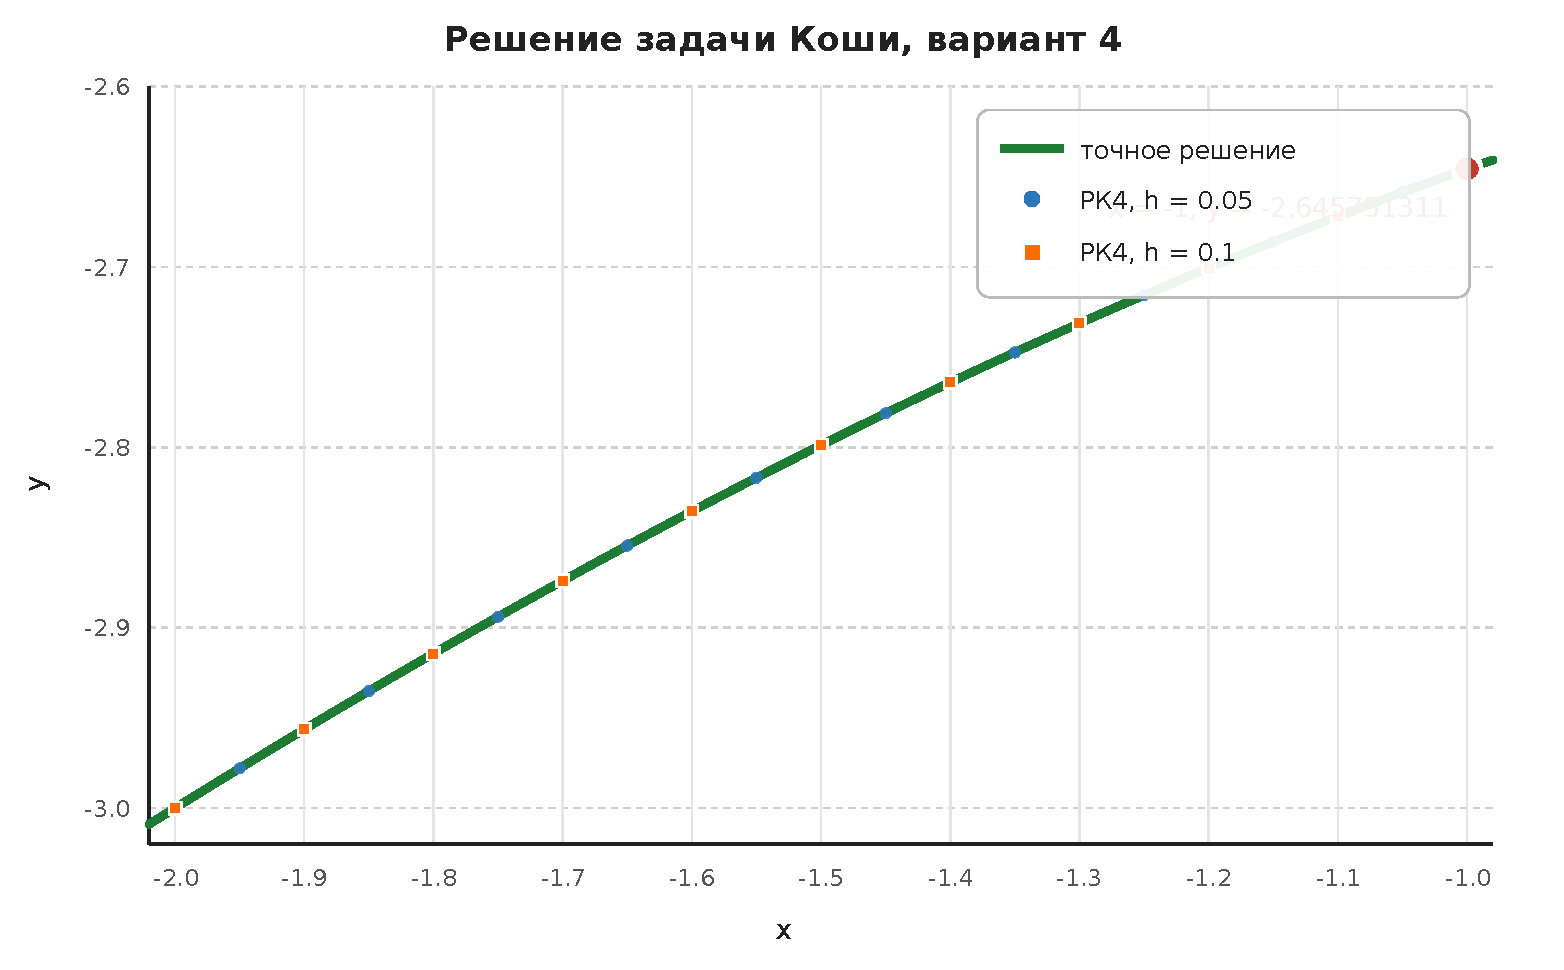
\includegraphics[width=0.9\textwidth]{fig_ode.pdf}
    \caption{Точное решение и численные решения РК4 для варианта~4}
    \label{fig:ode}
\end{figure}

% =====================================================================
\section{Обсуждение результатов}
% =====================================================================

Численное решение монотонно возрастает от $-3$ при $x=-2$ до
$-2{,}645751311$ при $x=-1$, что согласуется с точным решением
\eqref{eq:exact} и со знаком правой части: при $x<0$ и $y<0$
производная $y'=2x/(3y)$ положительна.

Отношение погрешностей на конце отрезка равно
\[
    \frac{|y_{0{,}1}-y|}{|y_{0{,}05}-y|}
    = \frac{3{,}55\cdot10^{-9}}{2{,}24\cdot10^{-10}}
    \approx 15{,}9 \approx 2^4 = 16,
\]
что подтверждает четвёртый порядок точности метода Рунге-Кутта.
Уменьшение шага вдвое снижает ошибку примерно в 16~раз.

Уточнение по правилу Рунге дало значение $-2{,}645751311062$, отличающееся
от точного всего на $2{,}2\cdot10^{-12}$, то есть примерно в 100~раз
точнее решения на мелкой сетке без уточнения. Наибольшая поправка
$3{,}32\cdot10^{-9}$ наблюдается в конце отрезка, где накопленная
погрешность максимальна; в начальной точке поправка равна нулю, так как
начальное условие задано точно.

Таким образом, цели работы достигнуты: метод Рунге-Кутта реализован,
решение задачи Коши получено на двух сетках, оценка погрешности по Рунге
подтверждена сравнением с точным решением \eqref{eq:exact}.

\end{document}
